% Build from this directory with tectonic MGS-KAN-Experimental-Report.tex.
% Alternatively, run pdflatex twice. Keep study-math.tex and report-figures/ here.
\documentclass[11pt]{article}
\usepackage[margin=1in]{geometry}
\usepackage{amsmath,amssymb,graphicx,booktabs,tabularx}
\usepackage[section]{placeins}
\usepackage[hidelinks]{hyperref}
\urlstyle{tt}

\newcolumntype{Y}{>{\raggedright\arraybackslash}X}
\newcolumntype{Z}{>{\raggedleft\arraybackslash}X}
\setlength{\parindent}{0pt}
\setlength{\parskip}{.45em plus .15em}
\setlength{\emergencystretch}{2em}
\setlength{\tabcolsep}{5pt}
\renewcommand{\arraystretch}{1.15}
\setcounter{tocdepth}{1}
\numberwithin{equation}{section}

\title{MGS-KAN and MLP Experimental Report\\[.5ex]
       \large Diploma project on sparse interactions and Gaussian geometry}
\author{}
\date{}

\begin{document}
\maketitle


\section{Summary}

This study compares a standalone MGS-KAN and a similarly sized MLP on sparse regression. It
measures scalar prediction, planted-pair recovery and interaction shape. In a separate
Gaussian-state benchmark, the seven-model rankings repeated on fresh data. MGS-KAN led on
nonlinear prediction and ranked fourth on geodesic.

The original 949-parameter MGS-KAN reduced test RMSE by \textbf{29.3\%} on the first sparse
target, from \textbf{0.3303} for the 937-parameter MLP to \textbf{0.2334}. The ten-seed
follow-up confirmed a substantial gain on that target and found a smaller gain on a second,
more oscillatory target. Exact pair recovery held on both sparse targets in the follow-up,
including the split where the MLP predicted more accurately.

The subsequent diagnosis isolated a large shape error on the oscillatory pair (2,4). In the
controlled study, increasing that pair from two to eight kernels lowered its error in
\textbf{all 36 matched comparisons} at both checkpoint endpoints. On ten entirely new data
seeds, the frozen targeted expansion had lower pair MSE and lower test RMSE than both original
models on \textbf{10/10 seeds}. The confirmation evaluated an expansion at a known pair on the
same synthetic function.

With a matched parameter budget, explicit triples improved prediction over
the pairwise geometry model on targets with a planted triple. The known
triple ranked first in all 30 hypergraph fits with a planted triple,
while Flat MLP achieved the lowest
prediction error. For the original geometry tasks, the advantage under
distribution shift depended on the shift. On held-out concrete mixtures,
the hypergraph model had a mean RMSE of 6.119 MPa, compared with 6.091 MPa
for the MLP.

\tableofcontents

\section{Research question and study design}

The primary question was whether an additive model with explicit Gaussian pair terms would
provide a prediction advantage for sparse interactions at a similar parameter count. The
experiment also asked whether the model could locate the pairs and estimate their shapes.
These last two questions use different criteria. A high estimated interaction magnitude can
identify a pair even when the fitted bivariate surface has substantial error.

\begin{center}
\small
\begin{tabularx}{\linewidth}{@{} >{\hsize=.60\hsize}Y>{\hsize=1.40\hsize}Y r @{}}
\toprule
\textbf{Stage} & \textbf{Design} & \textbf{Archived fits} \\
\midrule
Original study & Two targets \ensuremath{\times} three data seeds \ensuremath{\times} three initializations \ensuremath{\times} two models & 36 \\
Expanded follow-up & Three targets \ensuremath{\times} ten new data seeds \ensuremath{\times} three initializations \ensuremath{\times} two models & 180 \\
Shape diagnosis & Reanalysis of saved checkpoints for both sparse targets in the follow-up & 120 reused \\
Controlled fits & Three existing splits \ensuremath{\times} three initializations \ensuremath{\times} eight crossed settings & 72 \\
Fresh-seed confirmation & Second sparse target \ensuremath{\times} ten new data seeds \ensuremath{\times} three initializations \ensuremath{\times} three models & 90 \\
\bottomrule
\end{tabularx}
\end{center}

The original test seeds were 2311, 2411 and 2511. The follow-up seeds were 3301, 3307, 3313,
3319, 3323, 3329, 3331, 3343, 3347 and 3359. The controlled experiment used 3301, 3307 and
3313, the two closest follow-up seeds to 3307 plus the focus seed itself. The confirmation
used seeds 4101--4110. The same three initialization seeds, 71, 73 and 79, recur within each
data split. A data split is the independent unit for the paired prediction comparison. The
three initializations measure variation in training on the same rows.

\section{Models and synthetic targets}

\subsection{MGS-KAN and MLP architectures}

MGS-KAN sums an affine term, four univariate Gaussian kernels for each of 12 standardized
inputs, and two bivariate Gaussian kernels for each of the 66 unordered feature pairs. Every
bivariate kernel has a free amplitude, a two-coordinate center, and three free parameters in a
lower triangular factor. The diagonal entries are positive. For displacement d from the
center, each kernel is proportional to exp(\ensuremath{-}\ensuremath{\tfrac12}\(d^\top P d\)),
with P = \(LL^\top\). This allows rotated Gaussian surfaces. An individual pair contribution
is the sum of the kernels assigned to that pair. Training adds the sum of L2 norms of the pair
amplitude vectors, scaled by \ensuremath{\lambda}, to the mean squared error.

\begin{equation}
\begin{aligned}
\widehat y(z)
 &= b+w^\top z+
 \sum_{i=0}^{11}\sum_{k=1}^{4}a_{ik}
       \exp\!\left[-\tfrac12p_{ik}(z_i-c_{ik})^2\right]\\
 &\quad+\sum_{i<j}\sum_{k=1}^{2}a_{ijk}
       \exp\!\left[-\tfrac12d_{ijk}^\top L_{ijk}L_{ijk}^\top d_{ijk}\right].
\end{aligned}
\label{eq:report-scalar-model}
\end{equation}

Here z is the vector of standardized inputs, p is a positive univariate precision, and d is
the standardized pair input minus its kernel center.

The baseline has 13 affine parameters, 144 univariate parameters and 792 bivariate parameters,
for \textbf{949} total. The comparison MLP has two width-24 ReLU hidden layers and a scalar
linear output, for \textbf{937} parameters. The baseline counts differ by 1.26\% relative to
MGS-KAN. The targeted MGS-KAN changes only pair (2,4), adding six Gaussian kernels and 36
parameters for \textbf{985} total.

\subsection{Synthetic regression targets}

Each observation uses 12 independent standard-normal raw inputs. Feature indices are
zero-based. The shared additive components are \(\sin(x_6)\), \(0.5(x_7^2-1)\), and
\(\tanh(x_8)\). Each component is centered and scaled using a separate, fixed reference sample
of 100,000 rows. Their sum is centered and scaled again at the task level, then independent
Gaussian noise with standard deviation 0.10 is added. The training split alone sets the
feature means and scales used by the predictors.

\begin{center}
\small
\begin{tabularx}{\linewidth}{@{} l c Y @{}}
\toprule
\textbf{Target} & \textbf{Pair} & \textbf{Planted component before standardization} \\
\midrule
Original sparse & (0,1) & \(x_0x_1\) \\
Original sparse & (2,3) & \(\sin(x_2x_3)\) \\
Original sparse & (4,5) & Rotated Gaussian \\
Second sparse & (0,2) & \(\tanh(x_0)\tanh(x_2)\) \\
Second sparse & (1,5) & \(\exp[-\tfrac12((x_1-x_5)/0.6)^2]\) \\
Second sparse & (2,4) & \(\sin(2x_2)\sin(2x_4)\) \\
Additive control & --- & Shared additive components only \\
\bottomrule
\end{tabularx}
\end{center}

The rotated Gaussian uses the recorded substitute fixture with center (0.3,
\ensuremath{-}0.4), amplitude 1.7, principal axes rotated counterclockwise by \(\pi/6\), and
precision eigenvalues 4 and 0.5. The two sparse targets provide different shape and overlap
conditions. In the second target, pairs (0,2) and (2,4) share \(x_2\), and (2,4) changes sign
repeatedly along each input coordinate.

\section{Training and evaluation}

\subsection{Splits, paired training and checkpointing}

Each data seed produces 2,048 training, 512 validation and 2,048 test rows. Models share the
same split, observed targets and minibatch order within each data-seed and initialization
block. Tasks on the same data seed use the same raw inputs and noise draws. The test set is
scored after validation selects a checkpoint.

The optimizer is Adam with batches of 128. The standard runs validate every epoch for at most
300 epochs, use a patience of 30 epochs, and keep the earliest checkpoint at the lowest
validation RMSE. The original study compared four development settings per task and model by
crossing learning rates 0.001 and 0.003 with pair penalties 0.0001 and 0.001 for MGS-KAN, or
weight decay 0 and 0.001 for the MLP. It used development seed 2211. The follow-up inherited
these settings for the original targets and ran the same grid on development seed 3203 for the
second sparse target. The confirmation froze the expanded setting from the ablation before
seeing its fresh splits.

\begin{center}
\small
\begin{tabularx}{\linewidth}{@{} Y Z Z @{}}
\toprule
\textbf{Target} & \textbf{MGS-KAN LR / \ensuremath{\lambda}} & \textbf{MLP LR / weight decay} \\
\midrule
Original sparse & 0.003 / 0.001 & 0.003 / 0.001 \\
Additive control & 0.003 / 0.001 & 0.001 / 0.001 \\
Second sparse & 0.001 / 0.001 & 0.003 / 0 \\
Expanded arm on second sparse & 0.003 / 0.001 & --- \\
\bottomrule
\end{tabularx}
\end{center}

\subsection{Three evaluation measures}

\begin{enumerate}

\item \textbf{Whole-model test RMSE} uses noisy observed test targets and is in target units.
Results are averaged over the three per-fit RMSEs within each data seed before computing
paired differences.

\item \textbf{Interaction recovery} evaluates each MGS-KAN pair's pure interaction on the validation
rows. It subtracts the row and column means of the pair surface evaluated on the Cartesian
product of the empirical validation marginals, and adds the grand mean. The RMS along the
observed validation diagonal is the score. A pair is selected when its score strictly exceeds
5\% of the training-target standard deviation. Ranking and exact selection of the planted set
are reported separately.

\item \textbf{Pair shape MSE} measures squared error against the centered noiseless bivariate
surface and is in squared target units. It uses a common independent standard-normal input
measure. For an MLP, the comparable pair surface comes from the conditional mean of its whole
prediction. Shape errors are averaged across individual fits, with the same seed-level pairing
as above.

\end{enumerate}

Appendix~\ref{app:math} gives the definitions and derivations for all three measures.

\subsection{Checks before final evaluation}

The float64 checks cover all 66 unique pairs, decomposition of the prediction into its terms,
positive-definite precisions, numerical gradients, and interaction centering. The
rotated-Gaussian fixture matched the independent calculation to a maximum absolute error of
2.78 \ensuremath{\times} \(10^{-16}\). A 32-row noiseless overfit check with no regularization
passed for both models on all three targets. All six pilot training RMSEs were below
\(10^{-7}\), against a prespecified threshold of 0.05.

\section{Original study}

\subsection{Held-out prediction}

With 36 final fits, the baseline MGS-KAN had lower held-out RMSE on each of the three splits
for both targets. On the original sparse task, the mean of the seed-level RMSEs was
\textbf{0.2334} for MGS-KAN and \textbf{0.3303} for the MLP. On the additive control it was
\textbf{0.1164} and \textbf{0.1387}, respectively.

\begin{center}
\small
\begin{tabularx}{\linewidth}{@{} Y r r r r @{}}
\toprule
\textbf{Target} & \textbf{Seed} & \textbf{MGS-KAN RMSE} & \textbf{MLP RMSE} & \textbf{Difference} \\
\midrule
Original sparse & 2311 & 0.2313 & 0.3305 & \ensuremath{-}0.0992 \\
Original sparse & 2411 & 0.2292 & 0.3302 & \ensuremath{-}0.1010 \\
Original sparse & 2511 & 0.2398 & 0.3302 & \ensuremath{-}0.0904 \\
Additive control & 2311 & 0.1132 & 0.1365 & \ensuremath{-}0.0233 \\
Additive control & 2411 & 0.1243 & 0.1370 & \ensuremath{-}0.0127 \\
Additive control & 2511 & 0.1116 & 0.1426 & \ensuremath{-}0.0310 \\
\bottomrule
\end{tabularx}
\end{center}

Differences are MGS-KAN minus MLP, computed before rounding. The sparse-task RMSE of 0.2334
remains above the generator noise standard deviation of 0.10. The three consistent split-level
gains supported a broader replication.

\subsection{Interaction recovery}

All three planted pairs ranked in the top three and were the only selected pairs in
\textbf{9/9 original sparse fits}. The additive control selected zero pairs in
\textbf{9/9 fits}.

\section{Expanded follow-up}

\subsection{Held-out prediction}

The ten new splits reproduced the original sparse-target advantage. On the second sparse
target the mean advantage shrank to 0.0149 RMSE, and one split reversed direction. On that
split, seed 3307, MGS-KAN averaged 0.28831 and the MLP 0.27392.

\begin{center}
\small
\begin{tabularx}{\linewidth}{@{} Y Z Z Z Z @{}}
\toprule
\textbf{Target} & \textbf{MGS-KAN RMSE} & \textbf{MLP RMSE} & \textbf{Mean difference} & \textbf{MGS-KAN wins} \\
\midrule
Original sparse & 0.2403 & 0.3284 & \ensuremath{-}0.0881 & 10/10 \\
Second sparse & 0.2858 & 0.3007 & \ensuremath{-}0.0149 & 9/10 \\
Additive control & 0.1179 & 0.1386 & \ensuremath{-}0.0207 & 10/10 \\
\bottomrule
\end{tabularx}
\end{center}

\begin{center}
\small
\begin{tabularx}{\linewidth}{@{} l Z Z Z @{}}
\toprule
\textbf{Data seed} & \textbf{Original sparse \ensuremath{\Delta}} & \textbf{Second sparse \ensuremath{\Delta}} & \textbf{Additive \ensuremath{\Delta}} \\
\midrule
3301 & \ensuremath{-}0.0572 & \ensuremath{-}0.0124 & \ensuremath{-}0.0257 \\
3307 & \ensuremath{-}0.0777 & +0.0144 & \ensuremath{-}0.0169 \\
3313 & \ensuremath{-}0.0646 & \ensuremath{-}0.0138 & \ensuremath{-}0.0250 \\
3319 & \ensuremath{-}0.0841 & \ensuremath{-}0.0343 & \ensuremath{-}0.0249 \\
3323 & \ensuremath{-}0.1099 & \ensuremath{-}0.0410 & \ensuremath{-}0.0259 \\
3329 & \ensuremath{-}0.0993 & \ensuremath{-}0.0335 & \ensuremath{-}0.0156 \\
3331 & \ensuremath{-}0.0988 & \ensuremath{-}0.0104 & \ensuremath{-}0.0224 \\
3343 & \ensuremath{-}0.0701 & \ensuremath{-}0.0128 & \ensuremath{-}0.0216 \\
3347 & \ensuremath{-}0.1039 & \ensuremath{-}0.0028 & \ensuremath{-}0.0088 \\
3359 & \ensuremath{-}0.1152 & \ensuremath{-}0.0028 & \ensuremath{-}0.0199 \\
\bottomrule
\end{tabularx}
\end{center}

\subsection{Interaction recovery}

The original MGS-KAN recovered exactly the three planted pairs in \textbf{30/30 fits on the
original sparse target} and \textbf{30/30 on the second sparse target}. In each set of 30,
every planted pair ranked in the top three. None of the 66 candidate pairs crossed the cutoff
in any of the \textbf{30 additive-control fits}. Pair (2,4) was therefore recovered even in
the second-target fits on seed 3307. The ranking and selection results measure support
recovery. The shape analysis below evaluates how closely the learned surface follows the true
oscillations.

\section{Where the prediction gap narrowed}

\subsection{Estimating pure interaction error}

The post-hoc analysis reused 120 checkpoints from the two sparse tasks in the follow-up. For a
pair (i,j), it averaged each predictor conditionally over the remaining coordinates and
removed both marginal main effects and the grand-level contribution. It applied the same
centering to the true pair surface. MGS-KAN's architecture makes this centered surface
available directly from its assigned pair terms. The MLP projection used 256 scrambled Sobol
normal backgrounds. A 40-node Gauss--Hermite rule per coordinate integrated the squared
difference under the standard-normal product measure. A separate common sample of 32,768 Sobol
normal inputs estimated whole-model signal MSE against noiseless targets.

Here h is the conditional mean of the prediction for the fixed pair and g is its pure surface.

\begin{equation}
\begin{aligned}
g_{ij}(u,v)
 &=h_{ij}(u,v)
   -\mathbb E_{X_j}[h_{ij}(u,X_j)]
   -\mathbb E_{X_i}[h_{ij}(X_i,v)]\\
 &\quad+\mathbb E_{X_i,X_j}[h_{ij}(X_i,X_j)].
\end{aligned}
\label{eq:report-pair-projection}
\end{equation}

\begin{center}
\small
\begin{tabularx}{\linewidth}{@{} l Y r r @{}}
\toprule
\textbf{Target} & \textbf{Component} & \textbf{MGS-KAN pair MSE} & \textbf{MLP pair MSE} \\
\midrule
Original & Product (0,1) & 0.00988 & 0.00317 \\
Original & Sine of product (2,3) & 0.02632 & 0.04095 \\
Original & Rotated Gaussian (4,5) & 0.00074 & 0.00249 \\
Second & Tanh product (0,2) & 0.00478 & 0.00309 \\
Second & Gaussian ridge (1,5) & 0.00045 & 0.00143 \\
Second & Oscillatory product (2,4) & 0.05349 & 0.02712 \\
\bottomrule
\end{tabularx}
\end{center}

Under the independent input distribution, the pure pair components are orthogonal, including
the two components that share \(x_2\). The estimated MGS-KAN-minus-MLP gap in total noiseless
MSE moved from \ensuremath{-}0.04972 on the original target to \ensuremath{-}0.00832 on the
second, a shift of +0.04140 toward the MLP. The summed planted-pair gap shifted by +0.03675,
accounting for \textbf{89\% of that narrowing} in the estimated noiseless MSE gap. The largest
adverse pair difference on the second target was +0.02636 for (2,4). The remainder in the
decomposition includes unplanted and higher-order error and numerical integration error.

\subsection{The reversal on seed 3307}

On this split, the oscillatory pair MSE was \textbf{0.05565} for MGS-KAN and \textbf{0.02468}
for the MLP. The MLP's estimated remainder error, after accounting for the measured planted
pairs, first-order effects and squared mean bias, was also lower than on its other nine
splits, at 0.03238 versus 0.04078. Both factors narrowed the overall advantage.

\begin{center}
\small
\begin{tabularx}{\linewidth}{@{} Y r @{}}
\toprule
\textbf{Evaluation on seed 3307} & \textbf{MGS-KAN minus MLP} \\
\midrule
Noisy holdout MSE & +0.00796 \\
Noiseless target on the same holdout rows, MSE & +0.00702 \\
Independent normal inputs, noiseless signal MSE & +0.00587 \\
\bottomrule
\end{tabularx}
\end{center}

Initialization 73 drove the largest difference. Its noisy test RMSE was 0.2895 for MGS-KAN and
0.2586 for the MLP. Initialization 79 favored MGS-KAN on the independent noiseless draw. The
mean reversal persisted when the observation noise was removed. A denser 64-node projection
with 512 backgrounds kept the seed-3307 oscillatory pair gap positive at +0.03146, close to
the original +0.03098.

\begin{figure}[!htbp]
\centering
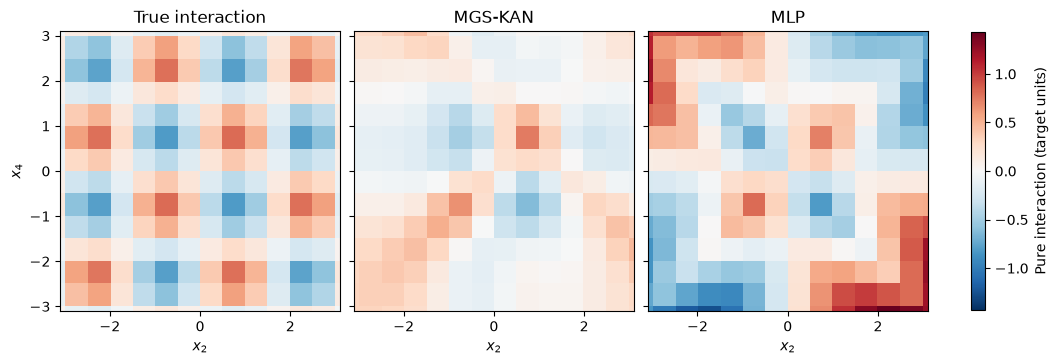
\includegraphics[width=\linewidth]{report-figures/seed-3307-oscillatory-pair.png}
\caption{True and fitted pure interaction surfaces for pair (2,4) on seed 3307. Fitted panels average
the three initializations for display. The error tables average losses from individual fits.}
\label{fig:oscillatory-pair}
\end{figure}

\section{Controlled fits on pair (2,4)}

\subsection{Factorial design}

The experiment crossed two or eight kernels on pair (2,4), Adam learning rates 0.001 or 0.003,
and group penalty \ensuremath{\lambda} = 0.001 or 0. Each of the eight configurations ran on
data seeds 3301, 3307 and 3313 with all three initializations. The two widths started with the
same predictor because the six additional kernels had zero starting amplitudes. Common
parameters, data and minibatch order were paired. Only the specified pair gained capacity. The
extra amplitudes joined its existing group penalty.

Each run retained two endpoints. The validation-selected checkpoint reproduced the original
selection and patience rule. Epoch 300 compared the same number of optimizer updates. The nine
replays at the original setting exactly reproduced their saved selected test predictions and
their validation histories through stopping.

\subsection{Matched effects}

Each contrast holds the other two factors, data seed and initialization fixed. A negative
change means the alternate level reduced error. The counts describe matched comparisons across
repeated settings and initializations on three splits.

\begin{center}
\small
\begin{tabularx}{\linewidth}{@{} >{\hsize=1.02\hsize}Y Z r >{\hsize=.98\hsize}Z r @{}}
\toprule
\textbf{Change} & \textbf{Mean \ensuremath{\Delta} pair MSE, selected} & \textbf{Lower} & \textbf{Mean \ensuremath{\Delta} pair MSE, epoch 300} & \textbf{Lower} \\
\midrule
2 \ensuremath{\to} 8 kernels & \ensuremath{-}0.03728 & 36/36 & \ensuremath{-}0.03739 & 36/36 \\
LR 0.001 \ensuremath{\to} 0.003 & \ensuremath{-}0.00355 & 28/36 & \ensuremath{-}0.00371 & 31/36 \\
\ensuremath{\lambda} 0.001 \ensuremath{\to} 0 & +0.00012 & 11/36 & +0.00001 & 15/36 \\
\bottomrule
\end{tabularx}
\end{center}

Kernel count had the largest and most consistent effect. On seed 3307 at \ensuremath{\lambda}
= 0.001, moving from two to eight kernels at the original learning rate reduced pair MSE from
\textbf{0.05565 to 0.02593}. Increasing the learning rate with two kernels changed the error
to \textbf{0.05559}. With eight kernels the same rate change reduced it further to
\textbf{0.01836}. The learning-rate benefit with eight kernels also appeared at epoch 300.
This pattern supports a capacity limitation for the two-kernel model under the tested
optimizer and training budget. The larger basis also benefited from the higher learning rate.

Removing the group penalty had a small mean effect on pair error. On seed 3307 it increased
whole-model test RMSE by \textbf{0.00512} on average across the matched validation-selected
comparisons. Across all three splits the corresponding increase was \textbf{0.00652}.

\begin{center}
\small
\begin{tabularx}{\linewidth}{@{} Y r r @{}}
\toprule
\textbf{Seed 3307, validation-selected} & \textbf{Pair MSE} & \textbf{Test RMSE} \\
\midrule
Original MGS-KAN, 2 kernels & 0.05565 & 0.28831 \\
8 kernels, original rate and penalty & 0.02593 & 0.21727 \\
8 kernels, LR 0.003, \ensuremath{\lambda} 0.001 & 0.01836 & 0.19236 \\
Saved MLP reference & 0.02468 & 0.27392 \\
\bottomrule
\end{tabularx}
\end{center}

The eight-kernel, 0.003 learning-rate, 0.001-penalty setting emerged from the explored splits.
A separate test on new data seeds then evaluated it with these settings frozen.

\begin{figure}[!htbp]
\centering
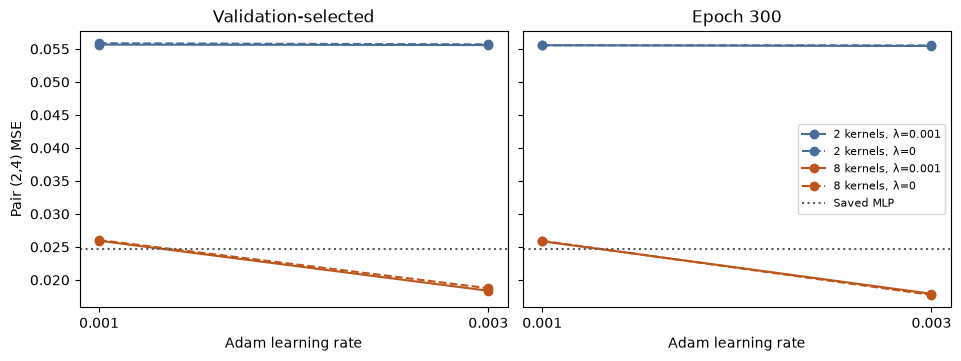
\includegraphics[width=\linewidth]{report-figures/seed-3307-controlled-fits.png}
\caption{Mean pair MSE on seed 3307 by learning rate, kernel count and group penalty. The horizontal
dotted line shows the saved MLP reference.}
\label{fig:controlled-fits}
\end{figure}

\section{Fresh-seed confirmation}

The confirmation compared 985-parameter expanded MGS-KAN, 949-parameter original MGS-KAN, and
937-parameter MLP on the second sparse target. The ten fresh splits and three initializations
per arm produced 90 fits. The original models retained their validated settings. The expanded
model used eight kernels on (2,4), learning rate 0.003 and \ensuremath{\lambda} = 0.001. The
validation rule and split structure carried forward.

\subsection{Pair (2,4) shape error}

\begin{center}
\small
\begin{tabularx}{\linewidth}{@{} Y r @{}}
\toprule
\textbf{Model} & \textbf{Mean pair MSE} \\
\midrule
Expanded MGS-KAN & \textbf{0.01533} \\
Original MGS-KAN & 0.05212 \\
MLP & 0.03182 \\
\bottomrule
\end{tabularx}
\end{center}

The expansion reduced pair error by \textbf{70.6\%} relative to original MGS-KAN and
\textbf{51.8\%} relative to the MLP. It had lower seed-level pair MSE on \textbf{10/10 splits
against each reference}. Expanded-minus-reference differences ranged from
\ensuremath{-}0.04448 to \ensuremath{-}0.03006 versus original MGS-KAN, and
\ensuremath{-}0.03629 to \ensuremath{-}0.00146 versus the MLP. A finer 64-node projection with
512 backgrounds preserved the direction on the three splits documented in the notebook. An
additional check applied that finer projection to all ten splits and retained the 10/10 result
against both references.

\subsection{Whole-model held-out prediction}

\begin{center}
\small
\begin{tabularx}{\linewidth}{@{} Y r @{}}
\toprule
\textbf{Model} & \textbf{Mean test RMSE} \\
\midrule
Expanded MGS-KAN & \textbf{0.18931} \\
Original MGS-KAN & 0.28447 \\
MLP & 0.30596 \\
\bottomrule
\end{tabularx}
\end{center}

The expansion reduced whole-model test RMSE by \textbf{33.5\%} relative to original MGS-KAN
and \textbf{38.1\%} relative to the MLP. It had lower seed-level test RMSE on \textbf{10/10
splits against each reference}. The mean paired differences were \ensuremath{-}0.09516 and
\ensuremath{-}0.11665 target units, respectively. The ten-seed ranges were
\ensuremath{-}0.12342 to \ensuremath{-}0.07350 against original MGS-KAN, and
\ensuremath{-}0.16117 to \ensuremath{-}0.07843 against the MLP.

\begin{figure}[!htbp]
\centering
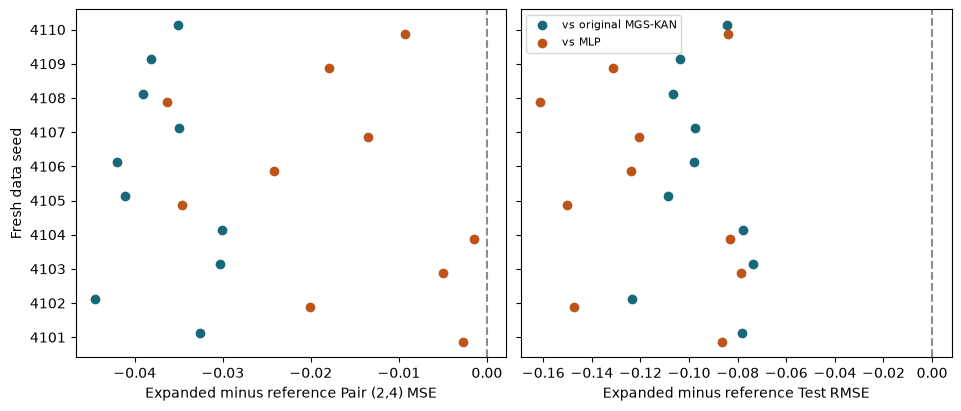
\includegraphics[width=\linewidth]{report-figures/fresh-seed-paired-differences.png}
\caption{All ten paired differences for pair shape MSE and whole-model test RMSE. The axes have
different units and scales. Negative values favor the expansion.}
\label{fig:scalar-confirmation}
\end{figure}

\section{Gaussian geometry prediction}

This benchmark predicts a bivariate Gaussian from two input Gaussians. It compares seven
models on affine, geodesic and nonlinear targets using mean squared Wasserstein distance
\(W_2^2\). The score is the sum of squared Euclidean center error and squared
Bures--Wasserstein covariance error. Scalar RMSE and planted-pair recovery are reported in the
preceding sections.

The original comparison used data seeds 3000, 4000 and 5000. The confirmation trained all
seven models on fresh seeds 6000, 7000 and 8000, with initializations 11, 29 and 47 on each
split, for 189 fresh fits. It retained the previous learning rates, architectures and float64
protocol. Each fit used 256 training cases, 128 validation cases, 256 test cases and 2,000
Adam updates. Checkpoint selection used the lowest validation \(W_2^2\). The fresh run used
CPU.

\subsection{Fresh held-out scores}

Mean test \(W_2^2\) \ensuremath{\times} \(10^3\), averaged over nine fits per task and model.
Bold marks the lowest error in each column.

\begin{center}
\small
\begin{tabularx}{\linewidth}{@{} Y r r r r @{}}
\toprule
\textbf{Model} & \textbf{Parameters} & \textbf{Affine} & \textbf{Geodesic} & \textbf{Nonlinear} \\
\midrule
MGS-KAN & 2,515 & 0.6156 & 1.5386 & \textbf{3.4113} \\
Flat MLP & 2,483 & 1.4958 & 2.5599 & 5.6751 \\
Spline / mean & 2,520 & \textbf{0.0177} & 3.5697 & 45.0840 \\
Spline / BW & 2,520 & 2.3578 & 1.1072 & 46.7395 \\
MLP edges / mean & 2,520 & 0.0288 & 1.4141 & 12.4486 \\
MLP edges / BW & 2,520 & 1.6024 & \textbf{0.3282} & 15.4990 \\
Anchor / BW & 162 & 5.9902 & 32.7037 & 64.9448 \\
\bottomrule
\end{tabularx}
\end{center}

The full ordering of the seven models repeated for all three tasks. MGS-KAN ranked third on
affine, fourth on geodesic and first on nonlinear. Its nonlinear test \(W_2^2\) was 39.9\%
below that of the runner-up, Flat MLP. It finished ahead of every nonlinear comparator on each
seed. It also beat Flat MLP on every affine and geodesic seed.

Paired MGS-KAN minus Flat MLP test \(W_2^2\) \ensuremath{\times} \(10^3\). Each difference
averages the three initializations within one data seed.

\begin{center}
\small
\begin{tabularx}{\linewidth}{@{} Y r r r @{}}
\toprule
\textbf{Data seed} & \textbf{Affine \ensuremath{\Delta}} & \textbf{Geodesic \ensuremath{\Delta}} & \textbf{Nonlinear \ensuremath{\Delta}} \\
\midrule
6000 & \ensuremath{-}1.0027 & \ensuremath{-}1.1294 & \ensuremath{-}2.9299 \\
7000 & \ensuremath{-}0.7729 & \ensuremath{-}0.9882 & \ensuremath{-}1.3918 \\
8000 & \ensuremath{-}0.8650 & \ensuremath{-}0.9463 & \ensuremath{-}2.4696 \\
\bottomrule
\end{tabularx}
\end{center}

\section{Why the geodesic gap persists}

The gap is in the covariance prediction. MGS-KAN averaged 0.00132446 covariance error versus
0.00002139 for MLP edges / BW. It averaged 0.00021416 center error versus 0.00030678 for that
model. The covariance excess exceeded the center advantage on all six seeds across the two
runs. The original mean \(W_2^2\) gap was +0.0011539.

Geodesic MGS-KAN minus MLP edges / BW test error \ensuremath{\times} \(10^3\).

\begin{center}
\small
\begin{tabularx}{\linewidth}{@{} Y r r r @{}}
\toprule
\textbf{Data seed} & \textbf{Center \ensuremath{\Delta}} & \textbf{Covariance \ensuremath{\Delta}} & \textbf{Total \ensuremath{\Delta}} \\
\midrule
6000 & \ensuremath{-}0.0372 & +1.0234 & +0.9862 \\
7000 & \ensuremath{-}0.1331 & +1.6440 & +1.5109 \\
8000 & \ensuremath{-}0.1076 & +1.2418 & +1.1342 \\
Mean & \ensuremath{-}0.0926 & +1.3031 & +1.2105 \\
\bottomrule
\end{tabularx}
\end{center}

\textbf{The target builds in covariance transport.} The true center is the ordinary weighted
average, with weights 0.65 and 0.35. The true covariance lies 35\% of the way along the
Bures--Wasserstein geodesic. Its transport matrix depends jointly on the two covariances,
including their relative orientations. Even an arithmetic covariance average with the correct
weights omits this transport.

\textbf{The architectures encode different operations.} The geometry version of MGS-KAN starts
from the arithmetic mean of the two Gaussian states, then predicts a residual in Cholesky
coordinates from the two encoded inputs. Its pairwise kernels must learn the correction to
that baseline. MLP edges / BW learns covariance transformations on its edges and combines the
resulting messages with Bures--Wasserstein barycenters. Its aggregation uses equal weights on
learned messages, so the task's 0.65/0.35 interpolation still has to be learned.

\textbf{The aggregation comparison supports this interpretation.} The two MLP-edge variants
share the same 2,520 parameters and geodesic learning rate of 0.01. With BW aggregation, mean
covariance error fell from 0.00100355 to 0.00002139, a 97.9\% reduction. The covariance error
improved on all three seeds. Under covariance-only shift, MLP edges / BW also led MGS-KAN,
with total \(W_2^2\) of 0.000697 versus 0.021992.

Geometry-aware aggregation is a plausible contributor to the lead. A matched MGS-KAN fit that
changes only its geometric baseline or aggregation would be needed to distinguish that effect
from differences in representation, regularization and optimization. Three new data seeds
support a descriptive comparison.

Geodesic and barycenter definitions follow Bhatia, Jain and Lim (2019).
\href{https://arxiv.org/abs/1712.01504}{On the Bures--Wasserstein distance between positive
definite matrices}

\section{Third-order hyperedges at a matched budget}
\label{sec:hyperedge-order}

\subsection{Scalar pilot}

The scalar pilot compared a full-coordinate kernel layer (I), a
singleton-and-pair layer (II), a singleton-pair-triple layer (III), and
a two-hidden-layer MLP. They had 515, 521, 517 and 516 trainable parameters,
respectively. I used 34 full-coordinate kernels. II used four kernels per
singleton and 13 per pair. III used four per singleton and per pair and
eight per triple. The MLP widths were \(4\to19\to20\to1\).
Four independent normal inputs drove an additive task, a
pure pair task and the pure triple \(u_0u_1u_3\), with standardized
\(u_i=\tanh(X_i)/\sqrt{\mathbb E[\tanh^2 X]}\) and independent response
noise of standard deviation \(0.1\). All models used the same splits and
minibatch order and trained without explicit regularization. Each task
used three paired data seeds and three initializations.

\textbf{Prediction.} The table gives the mean of the three per-fit test RMSEs
within each seed, then the mean across seeds.

\begin{center}
\small
\begin{tabularx}{\linewidth}{@{} Y r r r r @{}}
\toprule
\textbf{Task} & \textbf{I} & \textbf{II} & \textbf{III} & \textbf{MLP} \\
\midrule
Additive & 0.11590 & 0.10627 & 0.10763 & 0.11814 \\
Pair & 0.14007 & 0.13171 & 0.13650 & 0.12337 \\
Triple & 0.18937 & 1.02030 & 0.24996 & 0.15686 \\
\bottomrule
\end{tabularx}
\end{center}

On the triple task, III beat II on each seed. The population benchmark for
a sum of at most pairwise functions is \(\sqrt{1.01}\) RMSE, since the centered
triple is orthogonal to those functions. I and the MLP achieved lower test
RMSE than III on all three seeds. On the two lower-order controls, II
achieved lower RMSE than III on all three seeds.

\textbf{Recovery.} The planted triple \((0,1,3)\) ranked first among the
four groups in all nine III fits on the triple task. The largest triple
strength per run was \(0.00531\)--\(0.01036\) on the additive control and
\(0.02137\)--\(0.02601\) on the pair control. The scores use
\eqref{eq:triple-recovery} and there is no support-selection threshold.

\subsection{Geometry with a common residual and decoder}

All four geometry models encode two Gaussian states into ten scalar
coordinates and predict five residual coordinates relative to the encoded
arithmetic base. They share the Cholesky decoder in
\eqref{eq:gaussian-code}. Variant I uses 35 kernels on the full coordinate
set. II has three kernels per singleton and five per pair. III uses five
kernels per singleton and one per pair and per triple. Thus III includes
all 120 triples and reallocates capacity across orders. Each kernel has
a shared full precision and a five-vector amplitude. The parameter counts
are 2,505, 2,515, 2,535 and 2,483 for I, II, III and Flat MLP.

All four models were trained without explicit regularization. On
development seed 2000, each model and task used the same three-rate
grid and two initializations. The final 108 fits used fresh data seeds
9000, 10000 and 11000 and three matched initializations. Every fit
used 2,000 Adam updates and selected its checkpoint by validation \(W_2^2\).
The table reports test errors under the original generators.

\begin{center}
\small
\begin{tabularx}{\linewidth}{@{} Y l r r r @{}}
\toprule
\textbf{Task} & \textbf{Model} & \textbf{\(W_2^2\)} & \textbf{Center} & \textbf{Covariance} \\
\midrule
Affine & I & 0.0015233 & 0.0006717 & 0.0008517 \\
 & II & 0.0006423 & 0.0001549 & 0.0004873 \\
 & III & 0.0006305 & 0.0001489 & 0.0004816 \\
 & Flat MLP & 0.0014824 & 0.0006066 & 0.0008758 \\
Geodesic & I & 0.0031560 & 0.0013733 & 0.0017827 \\
 & II & 0.0012204 & 0.0003575 & 0.0008630 \\
 & III & 0.0012043 & 0.0002969 & 0.0009075 \\
 & Flat MLP & 0.0024804 & 0.0014122 & 0.0010682 \\
Nonlinear & I & 0.0089706 & 0.0046119 & 0.0043588 \\
 & II & 0.0042227 & 0.0013670 & 0.0028558 \\
 & III & 0.0041075 & 0.0014858 & 0.0026217 \\
 & Flat MLP & 0.0049898 & 0.0021732 & 0.0028167 \\
\bottomrule
\end{tabularx}
\end{center}

III had the lowest mean \(W_2^2\) in this four-model comparison and beat I
and Flat MLP on all nine task-by-seed comparisons. Its advantage over II
was small. III beat II on three of three affine, one of three geodesic
and two of three nonlinear splits. On geodesic it improved center error
on all three splits. Its covariance error increased enough to reverse
the total on seeds 10000 and 11000. On nonlinear it improved covariance
error on all three splits, with the larger center error reversing the
total on seed 10000.

\begin{figure}[!htbp]
\centering
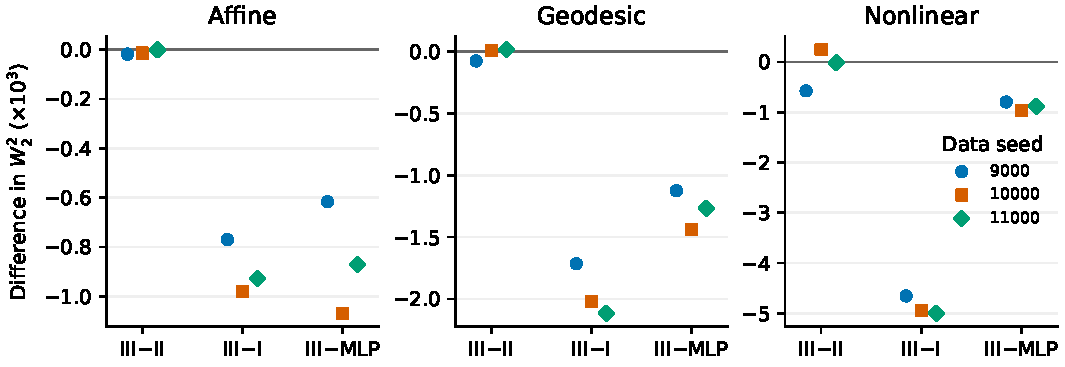
\includegraphics[width=\linewidth]{report-figures/geometry-order-paired-w2.pdf}
\caption{Paired test \(W_2^2\) differences for the geometry order comparison.
Each point averages three initializations within one data seed. Negative
values favor III. The panels use separate vertical scales.}
\label{fig:geometry-order-paired}
\end{figure}

\section{Distribution shifts with frozen weights}
\label{sec:geometry-shift}

The 108 geometry-order checkpoints were reloaded without retraining.
For each data seed the four conditions share a new set of base draws.
The center shift maps \(\mu\) to \(1.8\mu+(1,-0.6)^\top\).
The covariance shift adds \((0.5,-0.5)^\top\) to log standard deviations
in the sampled principal axes and keeps the angle fixed. The combined
condition applies both changes. Targets were regenerated on the shifted
inputs. The resulting 432 evaluations are matched to the unshifted
redraw rather than to the original test rows.

The first table gives mean \(W_2^2\). The second decomposes the paired
III-minus-II contrast and shows how much III's total error increased
relative to its own ID redraw.

\begin{center}
\small
\begin{tabularx}{\linewidth}{@{} Y l r r r r @{}}
\toprule
\textbf{Task} & \textbf{Model} & \textbf{ID redraw} & \textbf{Center shift} & \textbf{Covariance shift} & \textbf{Both shifts} \\
\midrule
Affine & I & 0.001716 & 0.017717 & 0.013418 & 0.030490 \\
 & II & 0.000736 & 0.009583 & 0.008076 & 0.016638 \\
 & III & 0.000717 & 0.009794 & 0.008173 & 0.017420 \\
 & Flat MLP & 0.001730 & 0.022779 & 0.012750 & 0.036446 \\
Geodesic & I & 0.003184 & 0.032405 & 0.028222 & 0.062617 \\
 & II & 0.001226 & 0.017741 & 0.016944 & 0.033385 \\
 & III & 0.001203 & 0.016852 & 0.017452 & 0.033765 \\
 & Flat MLP & 0.002584 & 0.034103 & 0.023902 & 0.058139 \\
Nonlinear & I & 0.008983 & 0.096210 & 0.027062 & 0.127475 \\
 & II & 0.004535 & 0.084343 & 0.012398 & 0.111666 \\
 & III & 0.004472 & 0.084873 & 0.011557 & 0.111493 \\
 & Flat MLP & 0.005208 & 0.103801 & 0.010381 & 0.130775 \\
\bottomrule
\end{tabularx}
\end{center}

\begin{center}
\small
\begin{tabularx}{\linewidth}{@{} Y l r r r r @{}}
\toprule
\textbf{Task} & \textbf{Condition} & \textbf{\(\Delta W_2^2\)} & \textbf{\(\Delta\) Center} & \textbf{\(\Delta\) Cov.} & \textbf{III vs.\ ID} \\
\midrule
Affine & ID redraw & -0.000018 & -0.000013 & -0.000005 & +0.000000 \\
 & Center shift & +0.000210 & +0.000161 & +0.000050 & +0.009077 \\
 & Covariance shift & +0.000097 & -0.000023 & +0.000120 & +0.007455 \\
 & Both shifts & +0.000782 & +0.000836 & -0.000054 & +0.016703 \\
Geodesic & ID redraw & -0.000022 & -0.000041 & +0.000018 & +0.000000 \\
 & Center shift & -0.000889 & -0.000984 & +0.000095 & +0.015649 \\
 & Covariance shift & +0.000508 & -0.000083 & +0.000591 & +0.016249 \\
 & Both shifts & +0.000380 & -0.000720 & +0.001100 & +0.032562 \\
Nonlinear & ID redraw & -0.000063 & +0.000069 & -0.000132 & +0.000000 \\
 & Center shift & +0.000530 & +0.002289 & -0.001759 & +0.080400 \\
 & Covariance shift & -0.000841 & -0.000061 & -0.000780 & +0.007085 \\
 & Both shifts & -0.000173 & +0.000314 & -0.000487 & +0.107021 \\
\bottomrule
\end{tabularx}
\end{center}

The relative order of II and III depends on the shift. On affine, II
leads III under all three shifts. On geodesic, III leads II under the
center shift, while II leads under the covariance and combined shifts.
On nonlinear, III leads II under the covariance and combined shifts.
Flat MLP has the lowest nonlinear covariance-shift \(W_2^2\) at 0.010381.
These comparisons concern prediction by frozen checkpoints.

\section{Gaussian targets with a known triple}
\label{sec:planted-geometry}

Two Gaussian inputs are decoded from scaled independent normal
coordinates. The generator adds a pure interaction of coordinates
\((0,2,8)\) to the first center coordinate or to the first log Cholesky
diagonal. A pair control uses \((0,2)\) and spreads its signal across
both outputs. Equation~\eqref{eq:planted-geometry} matches the total
population residual signal energy across the tasks. The splitting,
targets and batch order are paired across II, III and Flat MLP.

The development seed is 11991. The final data seeds are 12001, 12003,
12007, 12011 and 12013, with initializations 11, 29 and 47. Splits
contain 768 training, 256 validation and 1,024 test cases. The same
three-rate grid and the same 2,000-update schedule apply to each model.
The development and final stages comprise 54 and 135 fits.

\subsection{Prediction of center and covariance}

\begin{center}
\small
\begin{tabularx}{\linewidth}{@{} Y l r r r r @{}}
\toprule
\textbf{Task} & \textbf{Model} & \textbf{\(W_2^2\)} & \textbf{Center} & \textbf{Covariance} & \textbf{Residual RMSE} \\
\midrule
Center triple & II & 0.048501 & 0.048494 & 0.000007 & 0.220025 \\
 & III & 0.017373 & 0.017372 & 0.000001 & 0.130011 \\
 & Flat MLP & 0.000274 & 0.000269 & 0.000005 & 0.016430 \\
Covariance triple & II & 0.060859 & 0.000256 & 0.060603 & 0.226111 \\
 & III & 0.020310 & 0.000000 & 0.020310 & 0.129169 \\
 & Flat MLP & 0.000506 & 0.000003 & 0.000503 & 0.019491 \\
Pair control & II & 0.000155 & 0.000066 & 0.000089 & 0.011971 \\
 & III & 0.000112 & 0.000053 & 0.000060 & 0.010296 \\
 & Flat MLP & 0.000072 & 0.000031 & 0.000041 & 0.007840 \\
\bottomrule
\end{tabularx}
\end{center}

III reduced test \(W_2^2\) by 64.2\% relative to II on the center task
and 66.6\% on the covariance task. These improvements occurred on all
five seeds, predominantly in the component where the triple was
planted. III also beat II on all five pair-control splits. Flat MLP
had lower test \(W_2^2\) than III on every split of all three tasks.
Residual RMSE measures Euclidean error in the five encoded correction
coordinates, separately from the decoded Gaussian-state errors.

\subsection{Recovery of the planted triple}

The score in \eqref{eq:triple-recovery} measures the pure third-order
part of each of III's 120 explicit residual groups. Rank is based on
strength, with lexicographic tie-breaking.

\begin{center}
\small
\begin{tabularx}{\linewidth}{@{} Y r r @{}}
\toprule
\textbf{Task} & \textbf{Planted group at rank 1} & \textbf{Strength range} \\
\midrule
Center triple & 15/15 & 0.11941--0.18343 \\
Covariance triple & 15/15 & 0.10327--0.16679 \\
Pair control & --- & 0.00085--0.00163 \\
\bottomrule
\end{tabularx}
\end{center}

The true group ranked first in all 30 fits with a planted triple.
Its strength was below the population target strength \(0.22\).
The pair control gives the magnitude of the strongest estimated triple
in each fit. There is no selection threshold. The recovery result
establishes the ranking of the explicit groups on these synthetic
targets. Prediction accuracy is reported separately above.

\section{Concrete strength on unseen mixtures}
\label{sec:concrete-order}

The UCI Concrete Compressive Strength dataset contains 1,030 rows and
eight inputs \cite{yeh1998concrete}. An exact match on the seven ingredient
quantities defines a mixture group, giving 427 groups. All ages and
replicate rows of a mixture stay together. The five outer test folds
hold out disjoint groups. Validation uses 20\% of the remaining groups
within each fold. Age is transformed with \(\log(1+\mathrm{age})\).
Feature and target standardization use training rows only.

The scalar II, III and MLP have 993, 1,001 and 998 trainable parameters,
respectively. II uses six kernels per singleton and five per pair. III
uses four per singleton, two per pair and one per triple. The MLP widths
are \(8\to27\to26\to1\). Each outer fold uses the same three-rate search with two
development initializations, and three other initializations for the
final fits. The archive contains 90 validation runs and 45 final fits.
Test predictions are returned to MPa. The overall row for each model
averages three per-fit metrics within each fold and gives equal weight
to the five fold means.

\begin{center}
\small
\begin{tabularx}{\linewidth}{@{} Y r r r @{}}
\toprule
\textbf{Model} & \textbf{Parameters} & \textbf{RMSE (MPa)} & \textbf{MAE (MPa)} \\
\midrule
II & 993 & 6.226 & 4.685 \\
III & 1001 & 6.119 & 4.538 \\
MLP & 998 & 6.091 & 4.304 \\
\bottomrule
\end{tabularx}
\end{center}

\begin{center}
\small
\begin{tabularx}{\linewidth}{@{} l r Z Z Z @{}}
\toprule
\textbf{Fold} & \textbf{Test rows} & \textbf{II RMSE / MAE} & \textbf{III RMSE / MAE} & \textbf{MLP RMSE / MAE} \\
\midrule
1 & 176 & 6.628 / 5.113 & 6.497 / 5.028 & 6.217 / 4.638 \\
2 & 222 & 6.236 / 4.688 & 6.289 / 4.512 & 6.035 / 4.246 \\
3 & 234 & 6.852 / 5.014 & 6.511 / 4.722 & 6.946 / 4.485 \\
4 & 213 & 5.444 / 4.189 & 5.327 / 4.069 & 5.271 / 3.786 \\
5 & 185 & 5.969 / 4.423 & 5.969 / 4.361 & 5.985 / 4.364 \\
\bottomrule
\end{tabularx}
\end{center}

III improved mean RMSE by 0.107 MPa relative to II and had lower RMSE
on four folds. One of those differences, in fold 5, was below 0.001 MPa.
MLP had the lowest mean RMSE and MAE. Its mean RMSE was 0.028 MPa
below III, and its mean MAE was 0.235 MPa below III. This is evidence
about prediction on the five held-out folds of one dataset. The
dataset has no ground-truth interaction labels.

\section{What the evidence supports}

\textbf{Prediction at the original budget.} The original MGS-KAN delivered a consistent
advantage on the first sparse target over the nearly equal-size MLP. Its advantage was smaller
and less consistent on the second target. The second target's oscillatory interaction explains
a large share of the change in the measured noiseless error gap.

\textbf{Interaction recovery and shape.} The original architecture consistently detected the
planted support in these synthetic experiments. The additive control showed zero threshold
crossings across 39 original and follow-up fits. The large shape error on the detected
oscillatory pair shows why support recovery and shape fidelity warrant separate reporting.

\textbf{Targeted capacity.} The factorial study separates the capacity change from the tested
rate and group-penalty changes on three studied splits. Adding kernels produced the largest
pair-error improvement and retained that advantage with equal update counts. The frozen
expanded setting then improved both endpoints on independent splits drawn from the same second
target.

\textbf{Gaussian geometry prediction.} MGS-KAN's nonlinear lead repeated on fresh samples. On
the geodesic target, the strongest model was the MLP with Bures--Wasserstein aggregation, with
a clear advantage in covariance prediction. That seven-model comparison measured
prediction of Gaussian states.

\textbf{Third-order prediction.} In the controlled geometry tasks, III improved
both planted-triple predictions relative to II on all five splits. The advantage
over II on the standard geometry targets was smaller and sensitive to shifts.
Flat MLP led on the two planted-triple targets and the pair control. On concrete,
III had lower mean RMSE and MAE than II, while MLP had the lowest means.

\textbf{Third-order recovery.} III put the true triple first in all nine scalar
fits and in all 30 planted-geometry fits. The planted geometry score magnitude
remained below the target strength. Recovery of the explicit group and accuracy
of its fitted response therefore require separate measurements.

\textbf{Limits of the conclusion.} In the scalar pairwise studies, the inputs are independent
standard normals, the tasks are synthetic and the expanded pair was known from the generator.
The fresh-seed experiment varies
the samples while keeping the same target. Its comparison is between fixed settings, including
36 additional parameters and the higher learning rate in the expanded arm. The seed counts and
ranges are descriptive, and initializations on a single split share the same observations. A
procedure for choosing which unknown pair to expand and evidence across other target functions
remain open research questions.

\section{Reproducing the study}

The executable notebook contains the protocol, reports and plots. Run from the project root
with Python 3.12 and the dependencies pinned in \path{requirements-study.txt}. Restart the
Jupyter kernel and run all cells, or use the headless command.

\begin{verbatim}
python -m pip install -r requirements-study.txt
python -m jupyterlab study.ipynb
python -m nbconvert --to notebook --execute --inplace \
  --ExecutePreprocessor.timeout=-1 study.ipynb
\end{verbatim}

{\raggedright
The core implementation is in \path{src/config.py}, \path{src/data.py}, \path{src/models.py}
and \path{src/experiment.py}. The controlled and confirmation stages use
\path{experiments/pair_ablation.py} and \path{experiments/pair_confirmation.py}. Protocols
record seeds, settings and code fingerprints. Matching saved bundles are verified before
reuse. The full notebook reruns reproduced the corresponding tables and figures.\par}

\begin{center}
\small
\begin{tabularx}{\linewidth}{@{} >{\hsize=.5\hsize}Y>{\hsize=1.5\hsize}Y @{}}
\toprule
\textbf{Stage} & \textbf{Manifest path relative to the project root} \\
\midrule
Original study & \path{outputs/study/df24c2b5a1de3a48/final/manifest.json} \\
Expanded follow-up & \path{outputs/study/followup/9c04ad7dfc77dc19/final/manifest.json} \\
Controlled fits & \path{outputs/study/ablation/d7acbb7046e862ad/manifest.json} \\
Fresh-seed confirmation & \path{outputs/study/confirmation/8ef2c0ec02a44237/manifest.json} \\
\bottomrule
\end{tabularx}
\end{center}

The four manifests cover \textbf{378 fit files}, including nine baseline replays in the
ablation. The two endpoints per ablation fit bring the total to \textbf{450 saved test RMSEs}.
Independent recomputation from the archived predictions and targets matched to within 5.56
\ensuremath{\times} \(10^{-17}\) target units. The archived fit-file SHA-256 hashes also
matched. The development grid contributed 24 additional trials and the overfit check
contributed six pilot fits.

The recorded CPU is an Intel Core i5-9400F. In the original study the median training and
validation times per fit were 8.46 seconds for MGS-KAN and 3.45 seconds for the MLP. After an
interruption and cache reuse, the final original notebook invocation completed in 107.7
seconds. The follow-up took 330.3 seconds in its notebook invocation. The ablation and
confirmation stages took 163.8 and 159.2 wall seconds, respectively. These later runs used up
to five single-threaded workers, so their wall times describe execution of the stage rather
than summed training time.

{\raggedright
The geometry confirmation uses \path{experiments/geometry_confirmation.py}. Its
\path{manifest.json}, \path{individual_fits.csv} and \path{paired_differences.csv} are under
\path{outputs/study/geometry_confirmation/21f00c136f3672af/}. The completing CPU invocation
took 753 seconds after resuming two model groups. All 189 checkpoints reloaded, and an
independent recomputation matched all 1,323 split scores and their components to within 3.61
\ensuremath{\times} \(10^{-16}\). Two fresh Jupyter kernels reproduced the confirmation
tables.\par}

\subsection{Hypergraph run archives}

The following paths are relative to \path{outputs/study/}. Each archive
contains a protocol file and fit records. The shift archive references
the original geometry checkpoint digests. The concrete archive also
records the dataset SHA-256 and all grouped split assignments.

\begin{center}
\small
\begin{tabularx}{\linewidth}{@{} >{\hsize=.71\hsize}Y >{\hsize=1.29\hsize}Y r @{}}
\toprule
\textbf{Stage} & \textbf{Relative path} & \textbf{Final fits} \\
\midrule
Scalar order pilot & \path{hypergraph_order/2ce07e7736733605/} & 108 \\
Geometry order & \path{geometry_order/b160ed1b8a2f0af3/} & 108 \\
Frozen shifts & \path{geometry_shift/c99327eecfdbbe7d/} & 0 \\
Planted geometry & \path{planted_geometry/81762f947f7a54ec/} & 135 \\
Concrete mixtures & \path{concrete_order/bd2a1bf9045ef161/} & 45 \\
\bottomrule
\end{tabularx}
\end{center}

The geometry-order experiment verified 72 development and 108 final fits.
The first CPU invocation took 119.5 seconds for development and 181.2
seconds for final fitting and verification. The planted tasks took
111.3 and 270.4 seconds for 54 development and 135 final fits. Concrete
took 42.5 and 15.8 seconds for 90 development and 45 final fits.
The 432 shift evaluations reuse 108 final checkpoints.

Independent recomputation of geometry and shift scores matched all 945
split evaluations to within \(2.74\times10^{-16}\), including the center
and covariance components. The 5,400 geometry triple scores and ranks
were reproduced, as were RMSE and MAE for all 45 concrete fits. Two fresh
Jupyter kernels reproduced the follow-up tables.

\appendix

\section{Scalar fresh-seed results}

\label{app:scalar-results}

Each entry averages three fits for one data seed. The two tables use different units.

\subsection{Pair (2,4) MSE}

\begin{center}
\small
\begin{tabularx}{\linewidth}{@{} Y r r r @{}}
\toprule
\textbf{Data seed} & \textbf{Expanded MGS-KAN} & \textbf{Original MGS-KAN} & \textbf{MLP} \\
\midrule
4101 & 0.02328 & 0.05585 & 0.02599 \\
4102 & 0.00597 & 0.05045 & 0.02603 \\
4103 & 0.02625 & 0.05656 & 0.03125 \\
4104 & 0.02582 & 0.05587 & 0.02727 \\
4105 & 0.01105 & 0.05218 & 0.04562 \\
4106 & 0.01044 & 0.05248 & 0.03457 \\
4107 & 0.01578 & 0.05080 & 0.02925 \\
4108 & 0.01138 & 0.05041 & 0.04766 \\
4109 & 0.00776 & 0.04591 & 0.02569 \\
4110 & 0.01558 & 0.05071 & 0.02487 \\
\bottomrule
\end{tabularx}
\end{center}

\subsection{Test RMSE}

\begin{center}
\small
\begin{tabularx}{\linewidth}{@{} Y r r r @{}}
\toprule
\textbf{Data seed} & \textbf{Expanded MGS-KAN} & \textbf{Original MGS-KAN} & \textbf{MLP} \\
\midrule
4101 & 0.20491 & 0.28301 & 0.29123 \\
4102 & 0.15623 & 0.27965 & 0.30362 \\
4103 & 0.23171 & 0.30521 & 0.31014 \\
4104 & 0.20455 & 0.28242 & 0.28777 \\
4105 & 0.17991 & 0.28851 & 0.32995 \\
4106 & 0.18192 & 0.27974 & 0.30584 \\
4107 & 0.18909 & 0.28679 & 0.30979 \\
4108 & 0.18205 & 0.28858 & 0.34322 \\
4109 & 0.17132 & 0.27498 & 0.30249 \\
4110 & 0.19140 & 0.27577 & 0.27553 \\
\bottomrule
\end{tabularx}
\end{center}

\clearpage

\begingroup
\setlength{\parindent}{1.5em}
\setlength{\parskip}{0pt plus 1pt}
\setlength{\tabcolsep}{6pt}
\renewcommand{\arraystretch}{1}
\def\StudyReport{1}
% Standalone mathematical appendix. Compile with pdflatex (twice) or tectonic.
% Scalar sources: study.ipynb and src/{config,data,models,experiment}.py.
% Targeted fits: experiments/{pair_ablation,pair_confirmation}.py.
% Geometry: experiments/geometry_{reference,benchmark,confirmation}.py.
\documentclass[11pt]{article}
\usepackage[margin=1in]{geometry}
\usepackage{amsmath,amssymb,booktabs,url}

\newcommand{\E}{\mathbb{E}}
\newcommand{\R}{\mathbb{R}}
\newcommand{\N}{\mathcal{N}}
\newcommand{\SPD}{\operatorname{SPD}}
\newcommand{\tr}{\operatorname{tr}}
\newcommand{\sym}{\operatorname{sym}}
\newcommand{\norm}[1]{\lVert #1\rVert}
\newcommand{\setP}{\mathcal{P}}

\title{Mathematical Appendix for the MGS-KAN Experiments}
\author{}
\date{}

\begin{document}
\maketitle

The scalar studies compare prediction of noisy targets, recovery of planted
pair indices, and estimation of interaction surfaces. The Gaussian geometry
benchmark predicts a bivariate distribution and reports its center and
covariance errors. This appendix defines the quantities used in
\path{study.ipynb} and the experimental report.

\section{Scalar data generation}

An observation has raw features \(X=(X_0,\ldots,X_{11})^\top\) with independent
\(X_i\sim\N(0,1)\). The three shared additive components are
\[
 A(x)=\bigl(\sin x_6,\ \tfrac12(x_7^2-1),\ \tanh x_8\bigr).
\]
The following ordered component lists define the tasks. Concatenation with
\(A(x)\) retains its three entries.
\begin{align*}
 h_{\rm additive}(x) &= A(x),\\
 h_{\rm sparse}(x) &=
 \bigl(A(x),\ x_0x_1,\ \sin(x_2x_3),\ g_{\rm rot}(x_4,x_5)\bigr),\\
 h_{\rm overlap}(x) &=
 \biggl(A(x),\ \tanh x_0\,\tanh x_2,\
 \exp\!\left[-\tfrac12\left(\frac{x_1-x_5}{0.6}\right)^2\right],\
 \sin(2x_2)\sin(2x_4)\biggr).
\end{align*}
The planted sets are \(\varnothing\), \(\{(0,1),(2,3),(4,5)\}\),
and \(\{(0,2),(1,5),(2,4)\}\), respectively.

For the rotated Gaussian, the recorded substitute fixture uses
\(c=(0.3,-0.4)^\top\), amplitude \(1.7\),
\(\phi=\pi/6\), and principal precisions \(4\) and \(0.5\). Define
\begin{equation}
 R_\phi=\begin{pmatrix}\cos\phi&-\sin\phi\\\sin\phi&\cos\phi\end{pmatrix},
 \qquad P_\star=R_\phi\operatorname{diag}(4,0.5)R_\phi^\top .
 \label{eq:rotation}
\end{equation}
For \(d=(u,v)^\top-c\), the principal coordinates are \(q=R_\phi^\top d\).
Thus \(g_{\rm rot}(u,v)=1.7\exp[-(4q_1^2+0.5q_2^2)/2]\).

A separate reference sample of \(N_\star=100{,}000\) rows from NumPy's
\path{default_rng(101)}
sets the component statistics and the final target scale. Write
\(\E_\star\) for the reference sample average and \(t\) for the task:
\begin{align}
 m_{t,k}&=\E_\star[h_{t,k}(X)],&
 s_{t,k}^2&=\E_\star[(h_{t,k}(X)-m_{t,k})^2],\nonumber\\
 S_t(x)&=\sum_k \frac{h_{t,k}(x)-m_{t,k}}{s_{t,k}},&
 M_t&=\E_\star[S_t(X)],\qquad
 D_t^2=\E_\star[(S_t(X)-M_t)^2],\nonumber\\
 f_t(x)&=\frac{S_t(x)-M_t}{D_t},&
 Y_t&=f_t(X)+\varepsilon,\qquad
 \varepsilon\sim\N(0,0.1^2),\quad \varepsilon\perp X.
 \label{eq:target}
\end{align}
The components have equal weights after their individual standardization.
The normalization in \eqref{eq:target} gives the clean signal unit variance
on the reference sample, including when components share an input.

Each data seed supplies \(2048/512/2048\) train, validation, and test rows.
The tasks reuse the same raw inputs and noise draws within a data seed.
Models share the resulting split, observed targets, and example order.
For each feature, the model coordinate is
\[
 z_i=\frac{x_i-\widehat\mu_i}{\widehat\sigma_i},\qquad
 \widehat\mu_i=\frac{1}{n_{\rm tr}}\sum_{r\in{\rm tr}}x_{ri},\qquad
 \widehat\sigma_i^2=\frac{1}{n_{\rm tr}}\sum_{r\in{\rm tr}}
                    (x_{ri}-\widehat\mu_i)^2 .
\]
These scaling constants are fitted on the training rows and reused on the
other splits. The clean target and its components are available to the
evaluator.

\section{Scalar models and training}

Let \(\setP_d=\{(i,j):0\le i<j<d\}\) in lexicographic order.
The scalar MGS-KAN prediction decomposes as
\begin{align}
 \widehat y(z)
 &= b+w^\top z+\sum_{i=0}^{11}h_i(z_i)
      +\sum_{(i,j)\in\setP_{12}} g_{ij}(z_i,z_j),\label{eq:mgs}\\
 h_i(u)&=\sum_{k=1}^4 a_{ik}\exp[-p_{ik}(u-c_{ik})^2/2],
 \qquad p_{ik}=\exp(2\ell_{ik}),\nonumber\\
 g_{ij}(u,v)&=\sum_{k=1}^{K_{ij}} a_{ijk}
   \exp[-d_{ijk}^\top P_{ijk}d_{ijk}/2],
 \qquad d_{ijk}=(u,v)^\top-c_{ijk}.\nonumber
\end{align}
For every bivariate kernel, omitting indices, the implementation uses
\begin{equation}
 L=\begin{pmatrix}e^\alpha&0\\\beta&e^\gamma\end{pmatrix},
 \qquad P=LL^\top,\qquad
 d^\top P d=(e^\alpha d_1+\beta d_2)^2+(e^\gamma d_2)^2 .
 \label{eq:precision}
\end{equation}
The diagonal of \(L\) is positive, so \(L\) is invertible and
\(\norm{L^\top d}_2^2>0\) for \(d\ne 0\). The off-diagonal parameter
\(\beta\) allows the mixed term in the quadratic form.

Each of the \(66\) pairs has \(K_{ij}=2\) kernels in the baseline. A
univariate kernel uses one amplitude, one center and one log scale.
A bivariate kernel uses one amplitude, two center coordinates and three
precision-factor parameters. The counts are
\begin{align*}
 P_{\rm MGS}&=(12+1)+12\cdot4\cdot3+66\cdot2\cdot6=949,\\
 P_{\rm MLP}&=(12+1)24+(24+1)24+(24+1)=937,\\
 \frac{|P_{\rm MGS}-P_{\rm MLP}|}{P_{\rm MGS}}&=\frac{12}{949}
   \approx 1.26\% \le 5\%.
\end{align*}
The MLP is \(W_3\rho(W_2\rho(W_1z+b_1)+b_2)+b_3\), with both hidden widths
equal to \(24\) and \(\rho(u)=\max(u,0)\) elementwise.

For a minibatch \(B\), write
\(L_B(\theta)=|B|^{-1}\sum_{r\in B}(\widehat y_\theta(z_r)-y_r)^2\).
The MGS-KAN batch objective and the equivalent coupled weight-decay
objective for the MLP are
\begin{align}
 L_B^{\rm MGS}(\theta)
   &=L_B(\theta)+\lambda \sum_{(i,j)\in\setP_{12}}
           \norm{(a_{ijk})_{k=1}^{K_{ij}}}_2,\label{eq:penalty}\\
 L_B^{\rm MLP}(\theta)
   &=L_B(\theta)+\tfrac12\lambda_{\rm wd}\norm{\theta}_2^2.\nonumber
\end{align}
All candidate pairs can learn. The penalty acts on each complete amplitude
group in \eqref{eq:penalty}. For a nonzero group \(a\), its penalty gradient
is \(\lambda a/\norm{a}_2\).

Standard fits use Adam, batch size \(128\), and shuffled batches each epoch.
Validation occurs every epoch. For a split \(D\), define
\begin{equation}
 R_D(\theta)=
 \sqrt{\frac{1}{|D|}\sum_{r\in D}(\widehat y_\theta(z_r)-y_r)^2}.
 \label{eq:rmse}
\end{equation}
The selected epoch minimizes validation \(R_D\) among the evaluated
epochs, breaking ties at the earliest epoch. Training ends after
\(30\) epochs without improvement or \(300\) epochs in total.
The four development trials cross learning rates \(\{0.001,0.003\}\)
with MGS-KAN penalties \(\{10^{-4},10^{-3}\}\) or MLP weight decays
\(\{0,10^{-3}\}\). The task-specific choice minimizes validation RMSE.
The development seeds are \(2211\) for the original tasks and \(3203\)
for the second sparse target.

\begin{center}
\begin{tabular}{@{}lll@{}}
\toprule
Task & MGS-KAN \((\eta,\lambda)\) & MLP \((\eta,\lambda_{\rm wd})\)\\
\midrule
Original sparse & \((0.003,0.001)\) & \((0.003,0.001)\)\\
Additive control & \((0.003,0.001)\) & \((0.001,0.001)\)\\
Second sparse & \((0.001,0.001)\) & \((0.003,0)\)\\
\bottomrule
\end{tabular}
\end{center}

\paragraph{Numerical checks.}
The decomposition in \eqref{eq:mgs} reconstructs the forward result.
The float64 fixture checks all \(66\) pairs, symmetry and positive
eigenvalues of \(P\), and autograd against numerical derivatives for
inputs and parameters. For a scalar argument \(a\), the derivative used
in the numerical comparison is the centered difference
\([F(a+\delta)-F(a-\delta)]/(2\delta)\). A single nonzero kernel with
\(LL^\top=P_\star\) from \eqref{eq:rotation} must match evaluation in
the rotated coordinates, including off-axis displacements, with maximum
absolute error below \(10^{-10}\). A separate noiseless pilot uses \(32\)
rows, no regularization and a budget of \(350\) epochs. Its training
RMSE must be below \(0.05\) in unit-signal coordinates.

\section{Scalar prediction and recovery}

\subsection{Paired held-out prediction}

Let \(R_{m,s,r}\) denote test RMSE for model \(m\), data seed \(s\), and
initialization \(r\). With \(\mathcal I=\{71,73,79\}\) and data seeds
\(\mathcal S\), define
\begin{equation}
 \overline R_{m,s}=\frac{1}{|\mathcal I|}\sum_{r\in\mathcal I} R_{m,s,r},
 \qquad
 \Delta_s=\overline R_{{\rm MGS},s}-\overline R_{{\rm MLP},s},
 \qquad
 \overline\Delta=\frac{1}{|\mathcal S|}\sum_{s\in\mathcal S}\Delta_s .
 \label{eq:pair-average}
\end{equation}
A negative difference favors MGS-KAN. RMSE is computed per fit before the
averaging in \eqref{eq:pair-average}. The independent unit is the data seed.
When reported, relative reduction is \(1-\overline R_{\rm new}/\overline
R_{\rm ref}\), using the seed-averaged errors.

\subsection{Support recovery from validation marginals}

Fix a learned pair \(g_{ij}\) and the \(n_{\rm val}\) validation rows.
Let \(u_r=z_{ri}\), \(v_r=z_{rj}\), and
\(G_{rs}=g_{ij}(u_r,v_s)\). The empirical double-centering operator gives
\begin{align}
 \widetilde G_{rs}
 &= G_{rs}-\frac1n\sum_b G_{rb}-\frac1n\sum_a G_{as}
          +\frac1{n^2}\sum_{a,b}G_{ab},\qquad n=n_{\rm val},\nonumber\\
 S_{ij}&=\left(\frac1n\sum_{r=1}^n\widetilde G_{rr}^2\right)^{1/2},
 \qquad
 \widehat{\setP}
   =\{(i,j): S_{ij}>0.05\,\widehat\sigma_{Y,{\rm tr}}\}.
 \label{eq:validation-recovery}
\end{align}
The training-target standard deviation \(\widehat\sigma_{Y,{\rm tr}}\)
uses the noisy targets with divisor \(n_{\rm tr}\). The score and the
cutoff both have target units. The Cartesian product sets the marginal
means, while the diagonal evaluates the centered term on observed
validation pairs. If \(G_{rs}=a(u_r)+b(v_s)+c\), then
\(\widetilde G_{rs}=0\). If \(G_{rs}=u_rv_s\), then
\(\widetilde G_{rs}=(u_r-\bar u)(v_s-\bar v)\).

Pairs are ranked by descending \(S_{ij}\) with lexicographic tie-breaking.
If \(\setP_\star\) is the planted set, the reported top-three count is
\(\lvert\setP_\star\cap\operatorname{Top}_3(S)\rvert\).
Exact support recovery is \(\widehat{\setP}=\setP_\star\).
For the additive control, \(\lvert\widehat{\setP}\rvert\) counts false
selections.

\subsection{Population interaction shape error}

Here \(X\sim\N(0,I_{12})\) in raw coordinates. For a prediction function on
those coordinates \(F(x)=\widehat y(z(x))\), let
\(F_0=\E[F(X)]\) and \(F_i(u)=\E[F(X)\mid X_i=u]-F_0\).
The pure pair projection is
\begin{equation}
 F_{ij}(u,v)=\E[F(X)\mid X_i=u,X_j=v]-F_i(u)-F_j(v)-F_0 .
 \label{eq:conditional-projection}
\end{equation}
For a bivariate function \(b(u,v)\) and independent \(U,V\sim\N(0,1)\),
define
\[
 \mathcal C b(u,v)= b(u,v)-\E[b(u,V)]-\E[b(U,v)]+\E[b(U,V)] .
\]
For MGS-KAN the pair projection is exactly
\(\mathcal C[g_{ij}(z_i(\cdot),z_j(\cdot))]\), because conditional
expectations of other model terms contribute only constants and main
effects on these coordinates. For the MLP, \eqref{eq:conditional-projection}
uses its full prediction averaged over the remaining coordinates.
For the planted signal \(f_t\), the projected pair is the double-centered
version of its corresponding component divided by \(s_{t,k}D_t\).
For example, the oscillatory term on \((2,4)\) has zero population
marginal means by odd symmetry, giving
\[
 (f_{\rm overlap})_{24}(u,v)
   =\frac{\sin(2u)\sin(2v)}{s_{{\rm overlap},6}D_{\rm overlap}},
\]
where the component index \(k\) starts at one.
The constant subtracted in \eqref{eq:target} vanishes under projection.

For \(H\)-node Gauss--Hermite quadrature with nodes \(\xi_a\) and
weights \(\omega_a\) for \(e^{-x^2}\), the standard-normal nodes and
weights are \(x_a=\sqrt{2}\xi_a\) and \(w_a=\omega_a/\sqrt{\pi}\).
For a matrix \(B_{ab}=b(x_a,x_b)\), the discretization is
\begin{align}
 (\mathcal C_wB)_{ab}
   &=B_{ab}-\sum_\ell w_\ell B_{a\ell}
           -\sum_\ell w_\ell B_{\ell b}
           +\sum_{k,\ell}w_kw_\ell B_{k\ell},\nonumber\\
 \operatorname{PairMSE}_{ij}
   &=\E[(F_{ij}(U,V)-(f_t)_{ij}(U,V))^2]\nonumber\\
   &\approx \sum_{a,b}w_aw_b
      \bigl(F_{ij}(x_a,x_b)-(f_t)_{ij}(x_a,x_b)\bigr)^2 .
 \label{eq:pair-mse}
\end{align}
The primary diagnostic uses \(H=40\) and \(2^8\) common scrambled Sobol
background draws transformed by the standard-normal inverse CDF. The
finer check uses \(H=64\) and \(2^9\) backgrounds. Model inputs are
rescaled with each fit's training statistics before prediction. Shape
MSE has squared target units and uses a fixed product measure. The
validation RMS in \eqref{eq:validation-recovery} measures effect size.

\subsection{Noiseless error decomposition}

For \(e(x)=F(x)-f_t(x)\), let \(b=\E[e(X)]\) and
\(e_i(u)=\E[e(X)\mid X_i=u]-b\). Under the independent input measure,
constants, different centered main effects, and different pure pair
projections are mutually orthogonal in \(L^2\). For example, two pairs
sharing one feature have zero inner product because integrating a
nonshared coordinate gives zero. Consequently
\[
 \E[e(X)^2]
 =b^2+\sum_{i=0}^{11}\E[e_i(X_i)^2]
    +\sum_{(i,j)\in\setP_\star}\operatorname{PairMSE}_{ij} + E_{\rm rem}.
\]
The population remainder is the squared norm of components outside the
reported projections. The notebook estimates the total and bias on an
independent \(2^{15}\)-point scrambled Sobol draw, and computes the
numerical remainder by subtraction. Its value can include numerical
integration error. The population noisy MSE equals
\(\E[e(X)^2]+0.1^2\) by independence. On a finite test set the difference
between noisy and clean MSE also includes the empirical cross term
\(-2|D|^{-1}\sum_{r\in D}e(x_r)\varepsilon_r\).

\subsection{Targeted capacity experiment}

The expanded model has \(K_{24}=8\) and \(K_{ij}=2\) for every other
pair. Its six extra kernels start with zero amplitude and join the same
group in \eqref{eq:penalty}, so the initial prediction is unchanged.
The trainable count is \(949+6\cdot6=985\).

The crossed fit grid is
\[
 \mathcal H=\{2,8\}\times\{0.001,0.003\}\times\{0.001,0\},
\]
in the order kernel count, learning rate, and pair penalty.
For a factor \(k\), an endpoint and a metric \(M\), the matched effect
within a block \((s,r,h_{-k})\) is
\[
 \delta_k(s,r,h_{-k})
    =M(s,r,h_{-k},h_k^{\rm alternate})
     -M(s,r,h_{-k},h_k^{\rm original}).
\]
The report averages these differences over the \(3\cdot3\cdot4=36\)
matched blocks. One endpoint selects by validation with the usual
patience, and the other uses the checkpoint at epoch \(300\) for all
settings. The confirmation fixes the expanded arm at \((8,0.003,0.001)\)
and evaluates seeds \(4101\) through \(4110\). It compares
\(\operatorname{PairMSE}_{24}\) and whole-model \(R_D\) separately.

\section{Gaussian geometry benchmark}

\subsection{States, sampling, and metric}

A state is \(G=(\mu,C)\), with \(\mu\in\R^2\) and \(C\in\SPD(2)\).
Two input states are sampled independently. Per state, the center is
\(0.8\,Z\) with \(Z\sim\N(0,I_2)\), the angle \(\phi\) is uniform on
\([0,2\pi)\), and log standard deviations \(l\sim\N(0,0.35^2 I_2)\)
give \(C=R_\phi\operatorname{diag}(e^{2l_1},e^{2l_2})R_\phi^\top\).
The three draws are independent. The center shift maps
\(\mu\mapsto 1.8\mu+(1,-0.6)^\top\). The covariance shift maps
\(l\mapsto l+(0.5,-0.5)^\top\). Shifted test variants share the same
base draws with the unshifted redraw.

For another state \(H=(\nu,D)\), the prediction metric is
\begin{align}
 W_2^2(G,H)&=\norm{\mu-\nu}_2^2+d_{\rm BW}^2(C,D),\label{eq:w2}\\
 d_{\rm BW}^2(C,D)&=\tr C+\tr D-2\tr\bigl[(C^{1/2}DC^{1/2})^{1/2}\bigr].
 \nonumber
\end{align}
Matrix square roots are the positive definite ones. For independent
verification in dimension two, \(\tr(M^{1/2})=(\tr M+2\sqrt{\det
M})^{1/2}\) for \(M\in\SPD(2)\), since the two roots of the eigenvalues
sum to this expression. With \(M=C^{1/2}DC^{1/2}\), this gives
\begin{equation}
 d_{\rm BW}^2(C,D)=
 \tr C+\tr D-2\sqrt{\tr(CD)+2\sqrt{\det C\,\det D}} .
 \label{eq:w2-det}
\end{equation}
The implementation clamps small negative covariance errors caused by
roundoff to zero. Split scores average \(W_2^2\) and each component over
rows. The paired analysis then averages three training initializations
within each data seed, as in \eqref{eq:pair-average} with \(W_2^2\) in
place of RMSE.

\subsection{Three target maps}

For inputs \(G_i=(\mu_i,C_i)\), \(i=0,1\), write
\(\bar\mu=(\mu_0+\mu_1)/2\) and \(\bar C=(C_0+C_1)/2\).

\paragraph{Affine.}
For \(A=\left(\begin{smallmatrix}1.1&0.15\\0.15&0.85\end{smallmatrix}\right)\)
and \(b=(0.25,-0.15)^\top\), the target is
\[
 G_{\rm aff}=(A\bar\mu+b,\ A\bar C A^\top).
\]

\paragraph{Geodesic.}
The optimal transport matrix from \(C_0\) to \(C_1\) and the
interpolating covariance are \cite{bhatia2019}
\begin{align}
 T&=C_0^{-1/2}(C_0^{1/2}C_1C_0^{1/2})^{1/2}C_0^{-1/2},
       &T C_0T^\top&=C_1,\nonumber\\
 A_t&=(1-t)I+tT,& C_t&=A_t C_0 A_t^\top,\label{eq:geodesic}\\
 G_t&=((1-t)\mu_0+t\mu_1,\ C_t),& t&=0.35.\nonumber
\end{align}
Expanding the congruence in \eqref{eq:geodesic} gives
\begin{equation}
 (1-t)C_0+tC_1-C_t
    =t(1-t)(I-T)C_0(I-T)^\top\succeq 0 .
 \label{eq:arithmetic-gap}
\end{equation}
Even with the correct interpolation weights, an arithmetic covariance
average omits the transport correction. The benchmark MGS-KAN starts
from the equal-weight arithmetic average.

\paragraph{Nonlinear.}
Write \(u=(u_1,u_2)^\top=\mu_0\) and \(v=(v_1,v_2)^\top=\mu_1\).
Define
\[
 \delta(u,v)=\begin{pmatrix}0.35\sin(u_1v_2)\\0.30\tanh(u_2+v_1)\end{pmatrix},
 \qquad
 S(u,v)=\begin{pmatrix}
 0.18\sin(u_1+v_1)&0.12\tanh(u_2v_2)\\
 0.12\tanh(u_2v_2)&-0.15\cos(u_2-v_1)
 \end{pmatrix}.
\]
The target is \(G_{\rm nonlin}=(\bar\mu+\delta,\ e^S\bar C(e^S)^\top)\),
where \(e^S\) is the matrix exponential.

\subsection{Residual models for Gaussian states}

If \(C=LL^\top\) is its Cholesky factorization with positive diagonal,
define the encoding \(E\) and its inverse by
\begin{align}
 E(G)=(\mu_1,\mu_2,\log L_{11},L_{21},\log L_{22})^\top,\qquad
 &K(p,q,r)=\begin{pmatrix}e^p&0\\q&e^r\end{pmatrix},\nonumber\\
 E^{-1}(a_1,a_2,p,q,r)&=\bigl((a_1,a_2)^\top,\ K(p,q,r)K(p,q,r)^\top\bigr).
 \label{eq:gaussian-code}
\end{align}
Both residual models use a ten-coordinate input and a five-coordinate
output residual. With elementwise division by
\(s=(1.5,1.5,0.7,0.7,0.7)^\top\), their common form is
\[
 z=\begin{pmatrix}\tanh(E(G_0)/s)\\\tanh(E(G_1)/s)\end{pmatrix},
 \qquad
 \widehat G=E^{-1}\bigl(E(\bar\mu,\bar C)+r_\theta(z)\bigr).
\]
A zero residual returns the arithmetic base, and the decoder produces an
SPD covariance for finite coordinates in exact arithmetic.

Geometry MGS-KAN uses \eqref{eq:mgs}--\eqref{eq:precision} with \(10\)
input coordinates, \(3\) univariate kernels per coordinate, and \(5\)
bivariate kernels per pair over all \(45\) pairs. Every kernel has a
five-vector amplitude and a shared center and precision across the five
outputs. Flat MLP uses the same base and decoder, with a
\(10\to42\to42\to5\) network and two \(\tanh\) hidden activations.
The counts are
\begin{align*}
 P_{\rm geo,MGS}
   &=5(10+1)+10\cdot3(5+1+1)+45\cdot5(5+2+3)=2515,\\
 P_{\rm Flat}
   &=(10+1)42+(42+1)42+(42+1)5=2483.
\end{align*}

\subsection{Gaussian message models and aggregation}

The five message models use layer widths \(2\to3\to1\), giving nine
directed edges across the two layers. For the spline and MLP edge
variants, each edge \(j\to i\) maps
\(x=\tanh(E(G_j)/s)\) to \(q\in\R^5\). The messages are
\begin{align*}
 b&=(q_1,q_2)^\top,\qquad
 (\sigma_1,\sigma_2,\sigma_3)^\top=0.6\tanh((q_3,q_4,q_5)^\top/0.6),\\
 S&=\begin{pmatrix}\sigma_1&\sigma_2\\\sigma_2&\sigma_3\end{pmatrix},
 \qquad
 G_{ij}^{\rm msg}=(\mu_j+b,\ e^S C_j(e^S)^\top).
\end{align*}
The \(\tanh\) MLP edge is \(5\to25\to5\). A spline edge has
\(q_r=b_r+\sum_{a=1}^{5}\sum_{k=1}^{11}c_{rak}B_{k,3}(x_a)\).
The \(B_{k,3}\) are cubic B-splines on \([-1,1]\) with eight equal
intervals and repeated end knots. For knots \(\tau_k\), the recursion is
\[
 B_{k,0}(x)=\mathbf{1}_{[\tau_k,\tau_{k+1})}(x),\qquad
 B_{k,p}(x)=
 \frac{x-\tau_k}{\tau_{k+p}-\tau_k}B_{k,p-1}(x)
 +\frac{\tau_{k+p+1}-x}{\tau_{k+p+1}-\tau_{k+1}}B_{k+1,p-1}(x).
\]
Terms with zero denominator are set to zero. The coordinate spline and
MLP edges each have \(280\) parameters per edge, hence \(2520\) per
network. For Anchor / BW, each edge learns a state \(H\), a positive
scale \(\tau\), and a scalar cubic spline \(g\) on \([0,1]\).
Set \(r=W_2^2(G_j,H)/\tau^2\) and
\(t=(1+\exp[-g(r/(1+r))])^{-1}\); the message is the geodesic
interpolation from \(G_j\) to \(H\) at \(t\). With eleven coefficients
and one spline bias plus five state parameters and one log scale,
the count is \(9(11+1+5+1)=162\).

For incoming messages \(G_j^{\rm msg}=(\nu_j,D_j)\), let \(w_j=1/m\)
for \(m\) messages. Both aggregation rules use center \(\sum_jw_j\nu_j\).
Arithmetic aggregation uses covariance \(\sum_jw_jD_j\). BW aggregation
approximates the covariance barycenter
\[
 S_\star=\arg\min_{S\in\SPD(2)}\sum_j w_j d_{\rm BW}^2(S,D_j).
\]
Starting from \(S_0=\sum_jw_jD_j\), the benchmark applies twelve updates
\begin{align*}
 Q_\ell&=\sum_jw_j(S_\ell^{1/2}D_j S_\ell^{1/2})^{1/2},\\
 S_{\ell+1}&=\sym(S_\ell^{-1/2}Q_\ell^2S_\ell^{-1/2}),\qquad
 \sym(M)=(M+M^\top)/2 .
\end{align*}
The target in \eqref{eq:geodesic} is a weighted barycenter of the two
original inputs. The trained BW network uses equal weights on its learned
messages and learns their transformations.

\subsection{Geometry training and interpretation}

The batch objective is mean \(W_2^2\), with the additional penalty
\(0.001\sum_{(i,j)\in\setP_{10}}\norm{A_{ij}}_{\rm F}\) for MGS-KAN,
where \(A_{ij}\in\R^{5\times5}\) stacks the five kernel amplitude vectors
for the pair. The benchmark uses float64 Adam, minibatches of \(64\)
drawn with replacement, \(2000\) updates, gradient norm clipping at \(5\),
and train, validation and test sizes \(256/128/256\). Validation is
evaluated every \(10\) updates including step zero. The checkpoint is the
earliest minimizer of unpenalized validation mean \(W_2^2\).
For the batched Adam update, if \(g_t\) is the objective gradient at
update \(t\), the clipped gradient is
\(g'_t=g_t\min\{1,5/(\norm{g_t}_2+10^{-6})\}\).
With moments initialized to zero, the update is
\begin{align*}
 m_t&=\beta_1m_{t-1}+(1-\beta_1)g'_t,&
 v_t&=\beta_2v_{t-1}+(1-\beta_2)(g'_t)^2,\\
 \theta_t&=\theta_{t-1}
 -\eta\frac{m_t/(1-\beta_1^t)}
             {\sqrt{v_t/(1-\beta_2^t)}+10^{-8}},
 &(\beta_1,\beta_2)&=(0.9,0.999).
\end{align*}
The squares, square roots and divisions in the update are elementwise.
Scalar training uses the same Adam moment constants without clipping.
For the development selection, the score of a rate is the arithmetic
mean of the two initialization-specific best validation scores. Ties
favor the smaller rate.

The historical and fresh comparisons use data seeds
\(\{3000,4000,5000\}\) and \(\{6000,7000,8000\}\), respectively, with
training seeds \(\{11,29,47\}\) per data split. The fresh comparison
freezes the selected learning rates and pairs all seven models on the
same data and minibatch draws.

\begin{center}
\begin{tabular}{@{}lrrr@{}}
\toprule
Model & \multicolumn{3}{c}{Selected learning rate}\\
\cmidrule(l){2-4}
 & Affine & Geodesic & Nonlinear\\
\midrule
MGS-KAN          & 0.010 & 0.010 & 0.010\\
Flat MLP         & 0.003 & 0.001 & 0.010\\
Spline / mean    & 0.003 & 0.010 & 0.003\\
Spline / BW      & 0.010 & 0.010 & 0.001\\
MLP edges / mean & 0.010 & 0.010 & 0.010\\
MLP edges / BW   & 0.003 & 0.010 & 0.010\\
Anchor / BW      & 0.010 & 0.010 & 0.010\\
\bottomrule
\end{tabular}
\end{center}

The geodesic gap is measured by subtracting the two terms in
\eqref{eq:w2} separately. For MGS-KAN minus MLP edges / BW on the fresh
seeds, the mean center difference is \(-0.0000926\) and the covariance
difference is \(+0.0013031\), for \(+0.0012105\) total \(W_2^2\) after
rounding. The same MLP edge architecture with BW aggregation instead of
arithmetic aggregation reduced geodesic covariance error from
\(0.00100355\) to \(0.00002139\) at the same learning rate. Equation
\eqref{eq:arithmetic-gap} describes the correction implied by the target.
The aggregation comparison supports the geometric interpretation, and a
matched change within MGS-KAN would isolate its contribution.

\begin{thebibliography}{9}

\bibitem{bhatia2019}
R. Bhatia, T. Jain, and Y. Lim.
On the Bures--Wasserstein distance between positive definite matrices.
\emph{Expositiones Mathematicae}, 37(2), 165--191, 2019.
\url{https://doi.org/10.1016/j.exmath.2018.01.002}.

\end{thebibliography}

\end{document}

\endgroup

\end{document}
